% ============================================================
%  FINAL REPORT — Group 4
%  GraphRAG and Context Retrieval via Link Prediction
%  42913 Social and Information Network Analysis — Autumn 2026
%
%  HOW TO USE IN OVERLEAF:
%  1. Paste as main.tex (or compile this file directly)
%  2. Keep Imagens/ folder with UTS_logo.png and dashboard screenshots
%  3. Keep ../figures/ folder with the four analysis PNG figures
%  4. Compiler: pdfLaTeX  (Menu -> Compiler)
%  5. Click Recompile (twice for ToC)
% ============================================================

\documentclass[10pt]{article}

%% -- Packages -----------------------------------------------
\usepackage[english]{babel}
\usepackage[utf8]{inputenc}
\usepackage{amsmath}
\usepackage{amssymb}
\usepackage{graphicx}
\usepackage{color}
\usepackage{float}
\usepackage{caption}
\usepackage{subcaption}
\usepackage[margin=2cm]{geometry}
\usepackage{appendix}
  \renewcommand{\appendixname}{Appendices}
  \renewcommand{\appendixtocname}{Appendices}
  \renewcommand{\appendixpagename}{Appendices}
\usepackage[colorlinks=true,plainpages=true,citecolor=blue,linkcolor=blue]{hyperref}
\usepackage{fancyhdr}
  \pagestyle{fancy}
  \fancyhf{}
  \fancyhead[L]{\footnotesize 42913 Social and Information Network Analysis}
  \fancyhead[R]{\footnotesize GraphRAG Link Prediction --- Group 4}
  \fancyfoot[R]{\footnotesize Final Report}
  \fancyfoot[C]{\thepage}
  \fancyfoot[L]{\footnotesize Autumn 2026}
  \renewcommand{\footrulewidth}{0.4pt}
% booktabs replaced
\usepackage{tabularx}
\usepackage{longtable}
\usepackage[table]{xcolor}
\usepackage{array}
\usepackage{multirow}
\usepackage{tcolorbox}
  \tcbuselibrary{skins, breakable}
\usepackage{pgfplots}
  \pgfplotsset{compat=1.18}
\usepackage{tikz}
\usepackage{hanging}
\usepackage{titlesec}

%% -- Colours ------------------------------------------------
\definecolor{brandblue}{HTML}{1F3864}
\definecolor{accentblue}{HTML}{2E75B6}
\definecolor{lightblue}{HTML}{D6E4F0}
\definecolor{lightgray}{HTML}{F2F2F2}
\definecolor{midgray}{HTML}{CCCCCC}
\definecolor{darkgreen}{HTML}{1A6B1A}
\definecolor{warnorange}{HTML}{C55A11}
\definecolor{softgreen}{HTML}{E2F0D9}
\definecolor{softorange}{HTML}{FCE4D6}
\definecolor{ganttgreen}{HTML}{70AD47}
\definecolor{ganttblue}{HTML}{5B9BD5}
\definecolor{ganttorange}{HTML}{ED7D31}

%% -- Callout boxes ------------------------------------------
\newtcolorbox{callout}{
  enhanced,
  colback=lightblue,
  colframe=accentblue,
  leftrule=4pt, rightrule=0pt, toprule=0pt, bottomrule=0pt,
  arc=2pt, left=8pt, right=8pt, top=6pt, bottom=6pt,
  fontupper=\small
}

\newtcolorbox{limitbox}{
  enhanced,
  breakable,
  colback=softorange,
  colframe=warnorange,
  leftrule=4pt, rightrule=0pt, toprule=0pt, bottomrule=0pt,
  arc=2pt, left=8pt, right=8pt, top=6pt, bottom=6pt,
  fontupper=\small
}

\newtcolorbox{successbox}{
  enhanced,
  colback=softgreen,
  colframe=darkgreen,
  leftrule=4pt, rightrule=0pt, toprule=0pt, bottomrule=0pt,
  arc=2pt, left=8pt, right=8pt, top=6pt, bottom=6pt,
  fontupper=\small
}

\titleformat{\section}
  {\Large\bfseries\color{brandblue}}
  {\thesection}{0.7em}{}
  [\titlerule]
\titleformat{\subsection}
  {\large\bfseries\color{accentblue}}
  {\thesubsection}{0.7em}{}
\titleformat{\subsubsection}
  {\normalsize\bfseries\color{accentblue}}
  {\thesubsubsection}{0.7em}{}

%% -- Table helpers ------------------------------------------
\renewcommand{\arraystretch}{1.4}
\newcommand{\theadfont}{\bfseries\color{white}}

% ============================================================
\begin{document}
% ============================================================

%% -- Cover page --------------------------------------------
\begin{center}
\newcommand{\HRule}{\rule{\linewidth}{0.5mm}}

\begin{minipage}{0.48\textwidth}
  \begin{center}
    
\includegraphics[width=0.8\textwidth]{Imagens/UTS_logo}
  \end{center}
\end{minipage}

\vspace*{1.5cm}
\textsc{\huge 42913 Social and Information Network Analysis}\\[1.5cm]
\textsc{\LARGE Final Report}\\[1.5cm]
\vspace*{1.0cm}

\HRule\\[0.5cm]
{\Huge\bfseries GraphRAG and Context Retrieval}\\[0.2cm]
{\huge\bfseries via Link Prediction on the}\\[0.2cm]
{\huge\bfseries Wikipedia Vote Network}
\HRule\\[1.5cm]

\begin{minipage}{0.46\textwidth}
  \begin{flushleft}\large
    \emph{Authors:}\\
    Mitali Balki\\
    Ratticha Ratanawarocha\\
    Samriddhi Sud\\
    Shanessa Mascarenhas
  \end{flushleft}
\end{minipage}
\begin{minipage}{0.52\textwidth}
  \vspace{-0.6cm}
  \begin{flushright}\large
    \emph{Student ID:}\\
    25428006\\
    24996427\\
    25741149\\
    24632491
  \end{flushright}
\end{minipage}

\vspace{2cm}
{\large Group 4 $\cdot$ Topic 2 $\cdot$ \today}
\end{center}

\newpage

%% -- Abstract -----------------------------------------------
\textbf{\Huge Abstract}\\[0.4cm]

\bigskip
Large Language Models (LLMs) such as ChatGPT and Gemini have become widely used in many applications, but they still face a key limitation: they can hallucinate when they lack specific knowledge or access to private data. Retrieval-Augmented Generation (RAG) is a common solution that retrieves relevant documents to help the model answer correctly. However, standard RAG only works well for direct lookups and fails when the relationship between two entities is indirect. GraphRAG addresses this problem by organising knowledge as a graph, which allows the system to discover indirect connections through multi-hop path traversal.

This report presents a simplified GraphRAG retrieval module built on the Wikipedia Vote Network, a directed social trust graph from the Stanford Network Analysis Project (SNAP). The dataset contains 7,115 nodes and 103,689 directed edges. We frame context retrieval as a link prediction problem: if an algorithm predicts a strong link from user $A$ to user $B$, then $B$ is treated as relevant context for $A$. We implement and compare four network analysis algorithms: Common Neighbours, Jaccard Coefficient, Adamic/Adar Index, and Personalised PageRank.

The evaluation uses Precision@10 on a held-out 20\% test set with stratified negative sampling (10 negatives per positive edge). Personalised PageRank achieves the highest mean Precision@10 of \textbf{0.3369}, which is approximately 3.7 times better than a random baseline of 0.091. All four graph-based methods significantly outperform the random baseline, demonstrating that graph-structured retrieval can effectively surface indirect relationships that keyword-based search cannot find.

\begin{successbox}
\textbf{Key result.} Personalised PageRank (P@10 = 0.3369) outperforms all local similarity methods by approximately 11\% in relative terms and is 3.7$\times$ better than random guessing. This result confirms that multi-hop graph traversal is the most effective approach for indirect context retrieval in this network, directly supporting the core motivation of the GraphRAG approach.
\end{successbox}

\newpage
\tableofcontents
\newpage

% ============================================================
\section{Introduction}
\label{sec:intro}
% ============================================================

In recent years, Large Language Models (LLMs) such as ChatGPT, Gemini, and Claude have shown impressive performance in tasks like question answering, text summarisation, and code generation. However, these models have a fundamental limitation: their knowledge is fixed at the time of training, and they can only reason based on information given in the input prompt. When a question requires private, real-time, or highly specialised knowledge, LLMs often produce incorrect but confident-sounding responses, a problem commonly known as ``hallucination'' \cite{pan2024}.

\textbf{Retrieval-Augmented Generation (RAG)} \cite{lewis2020} was introduced to solve this problem by retrieving relevant documents from an external knowledge base and including them in the prompt before the model generates an answer. This approach works well for direct lookups. However, standard RAG relies on keyword matching or dense vector similarity, which fails when the relevant relationship between two entities is \emph{indirect}. For example, if a user asks ``How is the research of Professor~A indirectly influenced by the theories of Scientist~B?'', a keyword search will return nothing if A and B never co-authored or discussed each other directly. Yet the relationship A~$\rightarrow$~C~$\rightarrow$~B may clearly exist through an intermediate collaborator C.

\textbf{GraphRAG} \cite{edge2024} solves this by organising the knowledge base as a graph. Each node represents an entity (a person, paper, or concept) and each edge represents a relationship. Retrieving context becomes a graph traversal task: following edges to find relevant nodes, even across multiple hops. This allows the system to surface indirect relationships that flat retrieval would completely miss.

This project builds a simplified GraphRAG retrieval module using the \textbf{Wikipedia Vote Network}, a directed social trust graph where a directed edge from user~$i$ to user~$j$ means that user~$i$ voted for user~$j$ to become a Wikipedia administrator. If an algorithm predicts a strong link from user~$A$ to user~$B$, it means $B$ is treated as highly relevant context for $A$.

We implement and evaluate four link prediction algorithms:
\begin{itemize}
  \item Common Neighbours
  \item Jaccard Coefficient
  \item Adamic/Adar Index
  \item Personalised PageRank
\end{itemize}

Each algorithm produces a relevance score for each candidate pair. We evaluate performance using \textbf{Precision@10}: for each source node, we rank candidates by score and check how many of the top-10 predictions are real (held-out) edges.

The remainder of this report is organised as follows. Section~\ref{sec:related} discusses related work. Section~\ref{sec:dataset} describes the dataset. Section~\ref{sec:processing} explains the data processing steps. Section~\ref{sec:methods} presents the four algorithms. Section~\ref{sec:evaluation} defines the evaluation protocol. Section~\ref{sec:results} reports the experimental results. Section~\ref{sec:discussion} analyses the findings and discusses limitations. Section~\ref{sec:conclusion} concludes the report.

% ============================================================
\section{Related Work}
\label{sec:related}
% ============================================================

\subsection{GraphRAG}

Edge et al. \cite{edge2024} proposed GraphRAG as an extension of standard RAG for complex, multi-hop reasoning tasks. Their approach first extracts entities and relationships from documents to build a knowledge graph, then uses graph traversal to retrieve contextually relevant information. Unlike standard RAG, which retrieves documents based on vector similarity, GraphRAG can discover connections that span multiple degrees of separation. This is especially valuable for questions that require synthesising information across multiple sources.

\subsection{LLMs and Knowledge Graphs}

Pan et al. \cite{pan2024} provided a comprehensive roadmap for unifying LLMs and knowledge graphs (KGs). They argued that KGs can supply structured factual knowledge to LLMs, reducing hallucination and improving reasoning. They also identified link prediction as an important task for expanding and enriching knowledge graphs automatically.

\subsection{Link Prediction}

Liben-Nowell and Kleinberg \cite{libennowell2003} were among the first to study link prediction in social networks systematically. They compared several graph-based heuristics, including Common Neighbours, Jaccard, and Adamic/Adar, and found that graph structure alone provides useful information for predicting future edges. Their work established the evaluation framework (train/test split with Precision@K) that our project follows.

Adamic and Adar \cite{adamic2003} introduced the Adamic/Adar index, which weights shared neighbours by the inverse of their log-degree. This weighting scheme is motivated by the idea that being connected to a rare, niche hub provides stronger evidence of a relationship than being connected to a generic, high-degree hub.

\begin{callout}
\textbf{Project positioning.} Our work directly implements the retrieval module described in \cite{edge2024} as a link prediction benchmark. By comparing four different scoring algorithms on the Wikipedia Vote Network, we provide concrete, quantitative evidence for why graph-structured retrieval is more effective than keyword-based approaches for discovering indirect relationships.
\end{callout}

% ============================================================
\section{Dataset}
\label{sec:dataset}
% ============================================================

\subsection{Wikipedia Vote Network}

We use the \textbf{Wikipedia Vote Network} from the Stanford Network Analysis Project (SNAP) \cite{snap2014}. This dataset captures the administrator election process of Wikipedia, where editors can nominate and vote for other users to receive administrator privileges.

\begin{itemize}
  \item \textbf{Nodes:} Each node represents a unique Wikipedia user (editor), identified by an integer ID.
  \item \textbf{Edges:} A directed edge $i \rightarrow j$ means that user~$i$ voted for user~$j$, which is a direct signal of trust and relevance.
\end{itemize}

This network is well-suited for the GraphRAG retrieval task because:
\begin{enumerate}
  \item Edges encode trust, which is a natural proxy for relevance.
  \item The graph is sparse, so indirect paths are the main way two unconnected users are related.
  \item The hub-and-spoke structure means that a small number of highly-trusted administrators act as bridges between many ordinary users.
\end{enumerate}

\subsection{Dataset Statistics}

Table~\ref{tab:dataset} shows the key statistics of the Wikipedia Vote Network after cleaning (see Section~\ref{sec:processing}).

\begin{table}[H]
  \centering
  \caption{Wikipedia Vote Network statistics after data cleaning.}
  \label{tab:dataset}
  \begin{tabular}{lr}
    \hline
    \rowcolor{brandblue}
    \theadfont Property & \theadfont Value \\
    \hline
    \rowcolor{lightblue}
    Number of nodes                & 7,115 \\
    Number of directed edges       & 103,689 \\
    \rowcolor{lightblue}
    Graph density                  & 0.00205 \\
    Average in-degree              & 14.57 \\
    \rowcolor{lightblue}
    Average out-degree             & 14.57 \\
    Degree distribution            & Heavy-tailed (power-law-like) \\
    \hline
  \end{tabular}
\end{table}

The graph is \textbf{directed} because a vote flows from the voter to the candidate. It is \textbf{sparse}: only about 0.2\% of all possible directed pairs are connected. Despite this sparsity, the graph has a large weakly connected component, making link prediction a realistic and non-trivial task.

\subsection{Degree Distribution}

The degree distribution follows a heavy-tailed pattern, as shown in Figure~\ref{fig:degrees}. A small number of highly popular administrators receive thousands of votes, while the majority of users receive very few. This characteristic is common in real social networks and is important for understanding algorithm performance: high-degree hub nodes create short indirect paths between many pairs of users, which is the fundamental structure that graph-based methods can exploit.

\begin{figure}[H]
  \centering
  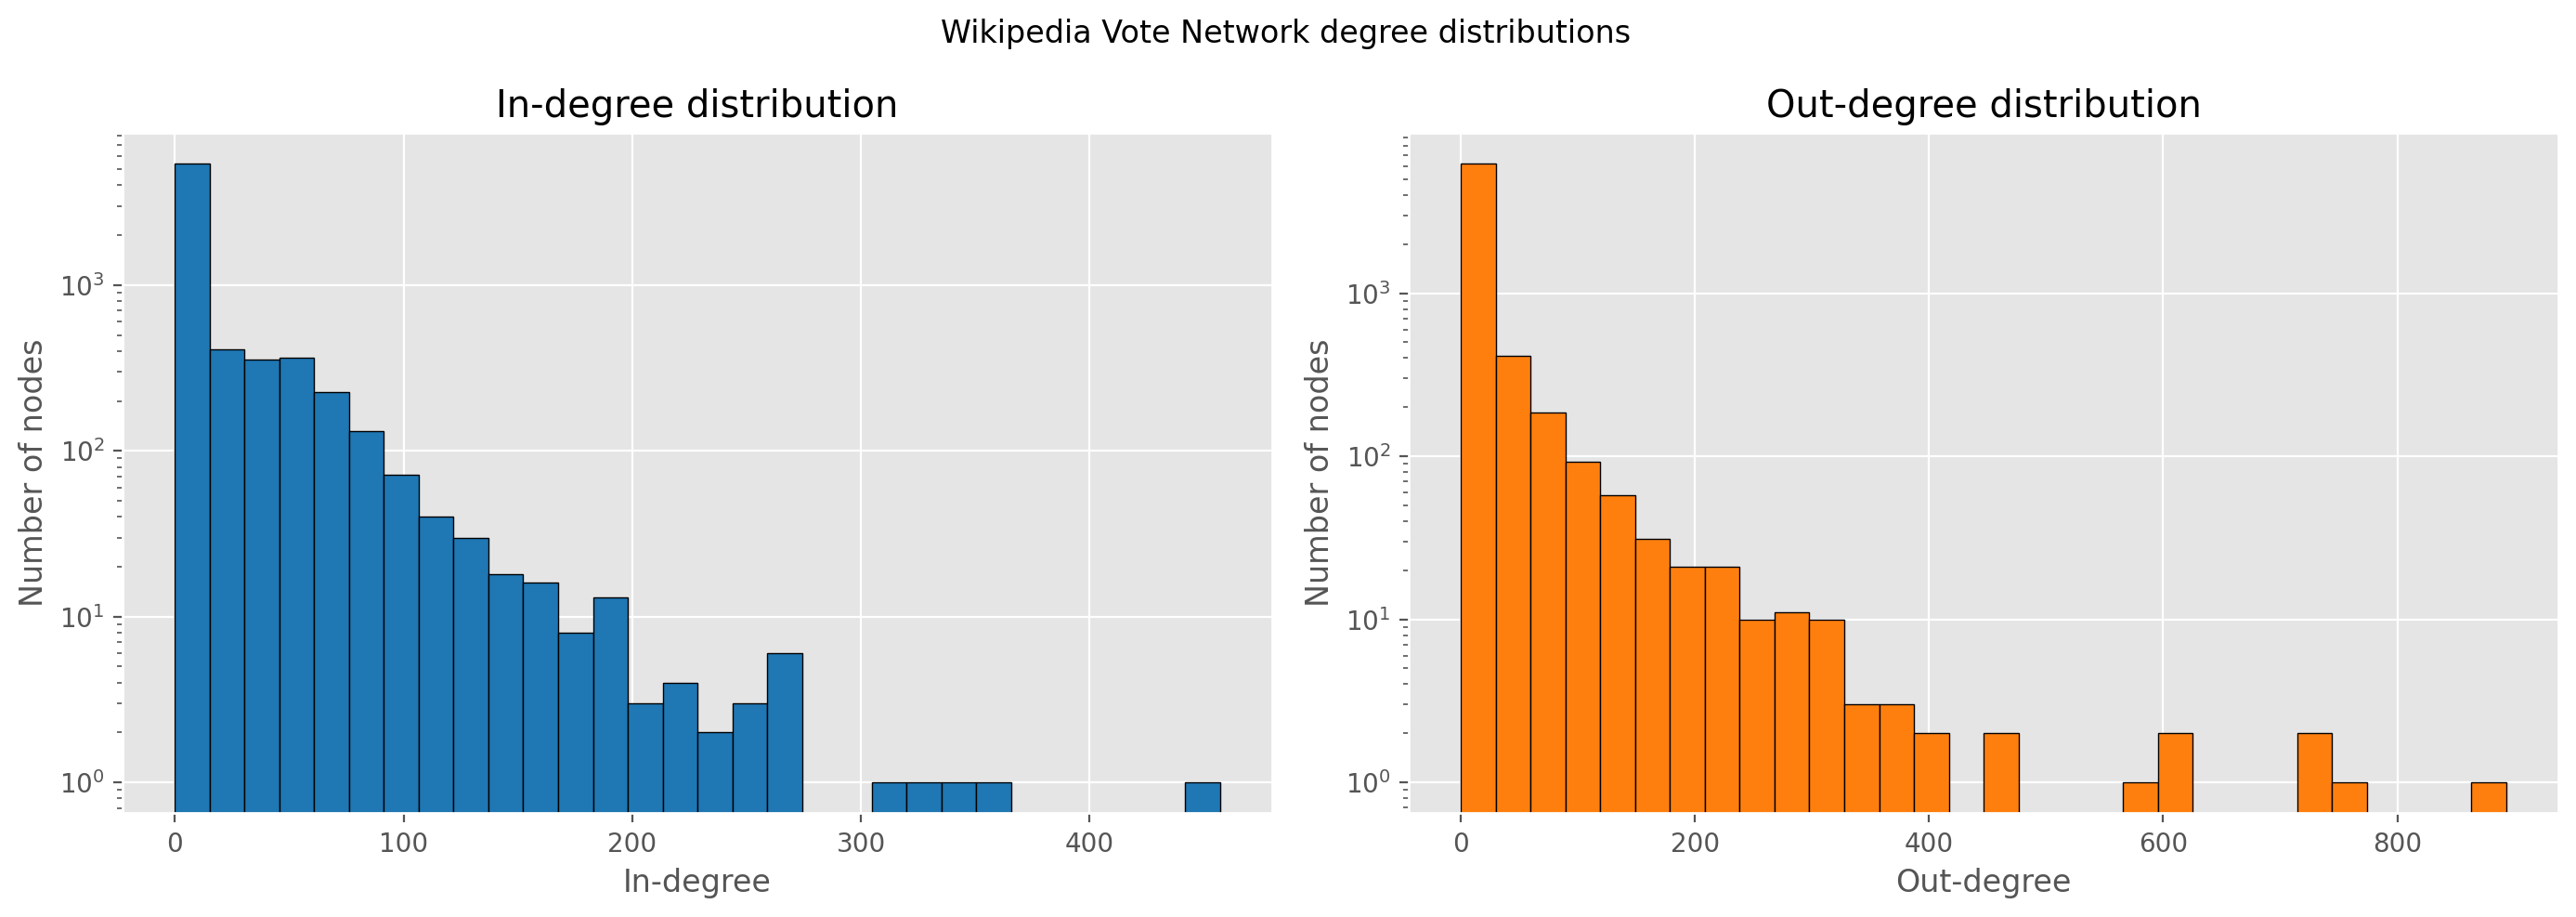
\includegraphics[width=0.92\textwidth]{../figures/degree_distributions}
  \caption{In-degree and out-degree distributions of the Wikipedia Vote Network (log-scale y-axis). Both distributions are heavy-tailed: a few administrators receive very high numbers of votes, while most users participate in only a few votes.}
  \label{fig:degrees}
\end{figure}

% ============================================================
\section{Data Processing}
\label{sec:processing}
% ============================================================

\subsection{Raw Data Format}

The SNAP file \texttt{wiki-Vote.txt} contains comment lines prefixed with \texttt{\#} (metadata about the graph) followed by pairs of integer user IDs separated by a tab character, with one directed edge per line. The dataset was downloaded programmatically from the SNAP website using the project script \texttt{scripts/download\_data.py}, which fetches the compressed \texttt{.gz} archive and extracts the text file automatically.

\subsection{Data Cleaning}

The raw edge list was processed using two cleaning steps:

\begin{enumerate}
  \item \textbf{Self-loop removal:} Edges where the source node equals the target node (i.e., a user voting for themselves) are removed. These edges carry no meaningful information for link prediction and do not appear in the real voting data.
  \item \textbf{Duplicate removal:} Repeated $(i, j)$ pairs are reduced to a single edge. In a directed graph, each ordered pair should appear at most once.
\end{enumerate}

After cleaning, the processed edge list contains \textbf{103,689 directed edges}, stored in \texttt{data/processed/graph\_edges.csv}.

\subsection{Train/Test Split Strategy}

We use a \textbf{random split} strategy with an 80\%/20\% ratio, following the standard approach for link prediction evaluation \cite{libennowell2003}:

\begin{enumerate}
  \item All cleaned edges are randomly shuffled using a fixed seed (42) to ensure reproducibility.
  \item The first 20\% of shuffled edges are reserved as the \textbf{test set}, representing the ``hidden'' ground truth that the algorithms must predict.
  \item The remaining 80\% form the \textbf{training set}, which is used to build the scoring graph.
  \item A \textbf{connectivity constraint} is enforced: an edge is only moved to the test set if both its source and target nodes still have at least one edge remaining in the training graph. This prevents isolated nodes, which would make scoring impossible.
\end{enumerate}

This design ensures that every node in the test set has a non-trivial neighbourhood in the training graph, making the evaluation fair and meaningful.

\subsection{Negative Sampling}

Standard link prediction evaluation requires both true positive edges (test edges) and \textbf{negative edges} (non-existent pairs) to create a realistic ranking scenario. Without negatives, any algorithm that assigns a positive score to all edges would achieve 100\% precision trivially.

For each source node in the test set, we sample \textbf{10 negative edges per positive test edge} from the space of non-existent directed pairs. Sampling is stratified by source node, ensuring that every evaluated node has the same ratio of positive to negative candidates. All sampled negatives are guaranteed not to exist in either the training or test sets.

\begin{table}[H]
  \centering
  \caption{Train/test split and candidate set statistics.}
  \label{tab:split}
  \begin{tabular}{lr}
    \hline
    \rowcolor{brandblue}
    \theadfont Set & \theadfont Edges \\
    \hline
    \rowcolor{lightblue}
    Training edges (80\%)          & 82,951 \\
    Test edges --- positive (20\%) & 20,738 \\
    \rowcolor{lightblue}
    Negative sampled edges         & 207,380 \\
    \hline
    Total candidate pairs scored   & 228,118 \\
    \rowcolor{lightblue}
    Source nodes evaluated         & 2,807 \\
    \hline
  \end{tabular}
\end{table}

% ============================================================
\section{Methods}
\label{sec:methods}
% ============================================================

All four algorithms are applied only to the \textbf{candidate set} (the union of positive test edges and sampled negative edges), not to all $7{,}115 \times 7{,}114 \approx 50$ million possible directed pairs. This is the standard efficiency approach recommended in the assignment specification and is sufficient for computing Precision@K accurately.

The three local similarity methods --- Common Neighbours, Jaccard, and Adamic/Adar --- operate on an \textbf{undirected projection} of the training graph. This treats the voting relationship as symmetric and allows the methods to count shared neighbours regardless of edge direction, which is appropriate for a social trust context. Personalised PageRank operates on the \textbf{directed training graph} to preserve the direction of trust flows.

\subsection{Common Neighbours}

For a pair of nodes $(u, v)$, the Common Neighbours score is the number of nodes that are direct neighbours of both $u$ and $v$ in the undirected training graph:

\begin{equation}
  \text{CN}(u, v) = |N(u) \cap N(v)|
  \label{eq:cn}
\end{equation}

\noindent\textbf{Intuition:} If user $A$ and user $B$ have both voted for (or been voted by) many of the same people, they are likely in the same community and are probably relevant to each other. In a GraphRAG context, if A and B are both connected to hub C, then C is the contextual bridge making B relevant to A.

\noindent\textbf{Limitation:} This method does not normalise for node degree, so high-degree hub nodes receive inflated scores regardless of actual relationship strength.

\subsection{Jaccard Coefficient}

The Jaccard Coefficient normalises the Common Neighbours count by the total number of distinct neighbours of either $u$ or $v$:

\begin{equation}
  \text{Jaccard}(u, v) = \frac{|N(u) \cap N(v)|}{|N(u) \cup N(v)|}
  \label{eq:jaccard}
\end{equation}

\noindent\textbf{Intuition:} A high proportion of shared neighbours (relative to all neighbours) indicates structural similarity. This metric is normalised, so it ranges between 0 and 1 and is not influenced by the absolute size of the neighbourhood.

\noindent\textbf{Limitation:} Normalising by the union heavily penalises high-degree nodes. In a social trust network, high-degree administrators are genuine connectors and their connections carry real information, so discounting them hurts performance.

\subsection{Adamic/Adar Index}

The Adamic/Adar Index \cite{adamic2003} assigns a weight to each shared neighbour based on the inverse of the logarithm of its degree:

\begin{equation}
  \text{AA}(u, v) = \sum_{w\; \in\; N(u) \cap N(v)} \frac{1}{\log |N(w)|}
  \label{eq:aa}
\end{equation}

\noindent\textbf{Intuition:} A shared neighbour that is itself low-degree (a niche, specialised user) provides stronger evidence of a direct relationship between $u$ and $v$ than a high-degree hub that is connected to nearly everyone. The log-weighting discounts these generic hubs. This is a refined version of Common Neighbours.

\noindent\textbf{In practice:} In this graph, Common Neighbours and Adamic/Adar produce nearly identical results because the heavy-tailed degree distribution means that most shared neighbours are already medium-degree nodes where $\log(\text{degree})$ values are similar.

\subsection{Personalised PageRank}

Personalised PageRank (PPR) \cite{page1999} computes a stationary probability distribution over the entire directed training graph, starting from a specific source node $u$. The teleportation vector is set so that all probability mass restarts at $u$ with probability $(1-\alpha)$, and the iteration is run with damping factor $\alpha = 0.85$:

\begin{equation}
  \mathbf{r}_u = \alpha\, \mathbf{A}^\top\, \mathbf{r}_u \;+\; (1 - \alpha)\, \mathbf{e}_u
  \label{eq:ppr}
\end{equation}

\noindent where $\mathbf{A}$ is the column-normalised adjacency matrix of the directed training graph and $\mathbf{e}_u$ is the one-hot vector for source node $u$. The relevance score for a candidate target $v$ is the probability mass $r_u(v)$ in the converged distribution.

\noindent\textbf{Intuition:} Think of a random walker who starts at user $A$, follows directed ``voted-for'' edges at each step, and occasionally (with probability $1-\alpha$) teleports back to $A$. After many steps, nodes reachable from $A$ via short, well-traversed paths accumulate higher probability mass and are therefore considered more relevant. Unlike the three local methods, PPR naturally captures \textbf{multi-hop indirect paths} and uses the \textbf{global structure} of the graph.

\noindent\textbf{Why it wins for GraphRAG:} The core value of GraphRAG is finding indirect relationships. PPR is the only method in this comparison that can directly follow a two-hop or three-hop path and assign a meaningful score to the endpoint --- precisely the capability that GraphRAG requires.

\begin{callout}
\textbf{Summary of method differences.} Common Neighbours, Jaccard, and Adamic/Adar all compute scores based only on \emph{one-hop} shared neighbours. They cannot assign a non-zero score to pairs that share no direct neighbours. Personalised PageRank follows multi-hop paths on the directed graph and can assign positive scores to nodes that are several hops away, which is the critical capability for discovering indirect relationships.
\end{callout}

% ============================================================
\section{Evaluation Setup}
\label{sec:evaluation}
% ============================================================

\subsection{Precision@K}

For each source node $u$, the algorithm ranks all candidate pairs $(u, *)$ by their computed score in descending order and recommends the \textbf{Top-$K = 10$} most likely links. The evaluation metric is:

\begin{equation}
  \text{Precision@}K(u) = \frac{\bigl|\{\text{Top-}K \text{ predictions for } u\} \cap \{\text{true test edges from } u\}\bigr|}{K}
  \label{eq:precision}
\end{equation}

The primary reported result is the \textbf{mean Precision@10} across all 2,807 evaluated source nodes.

\subsection{Why Precision@K Is Appropriate for GraphRAG}

In a real GraphRAG retrieval pipeline, the system selects the $K$ most relevant context nodes to inject into the LLM prompt. The quality metric is: how many of those $K$ selected nodes are genuinely relevant? Precision@$K$ measures exactly this. A higher Precision@10 means the GraphRAG engine retrieves better-quality context, which directly reduces the chance that the LLM will hallucinate an answer.

\subsection{Random Baseline}

A random algorithm that selects 10 candidates uniformly at random would achieve the following expected Precision@10:

\[
\frac{20{,}738 \;\text{positives}}{228{,}118 \;\text{total candidates}} \;\approx\; 0.091
\]

All graph-based algorithms must substantially exceed this value to justify the extra complexity of graph-based retrieval.

\subsection{Parameter Settings}

\begin{table}[H]
  \centering
  \caption{Experiment parameter settings used for all runs.}
  \label{tab:params}
  \begin{tabular}{ll}
    \hline
    \rowcolor{brandblue}
    \theadfont Parameter & \theadfont Value \\
    \hline
    \rowcolor{lightblue}
    Test fraction                   & 0.20 (20\%) \\
    Negatives per positive edge     & 10 \\
    \rowcolor{lightblue}
    Top-$K$                         & 10 \\
    PageRank damping factor $\alpha$ & 0.85 \\
    \rowcolor{lightblue}
    Random seed                     & 42 \\
    \hline
  \end{tabular}
\end{table}

% ============================================================
\section{Results}
\label{sec:results}
% ============================================================

\subsection{Precision@10 Summary}

Table~\ref{tab:results} shows the mean Precision@10, standard deviation, total true positive hits, and performance relative to the random baseline for all four methods and the random baseline.

\begin{table}[H]
  \centering
  \caption{Precision@10 results on the Wikipedia Vote Network test set (2,807 source nodes evaluated).}
  \label{tab:results}
  \begin{tabular}{l c c c c}
    \hline
    \rowcolor{brandblue}
    \theadfont Method &
    \theadfont Mean P@10 &
    \theadfont Std Dev &
    \theadfont Total Hits &
    \theadfont vs.\ Random \\
    \hline
    \rowcolor{softgreen}
    \textbf{Personalised PageRank} & \textbf{0.3369} & 0.2389 & 9,456 & $3.7\times$ \\
    Common Neighbours              & 0.3029 & 0.2328 & 8,502 & $3.3\times$ \\
    \rowcolor{lightblue}
    Adamic/Adar                    & 0.3027 & 0.2320 & 8,496 & $3.3\times$ \\
    Jaccard                        & 0.2941 & 0.2320 & 8,254 & $3.2\times$ \\
    \hline
    \rowcolor{lightgray}
    \textit{Random (baseline)}     & \textit{$\approx$0.091} & --- & --- & $1.0\times$ \\
    \hline
  \end{tabular}
\end{table}

\textbf{Personalised PageRank} achieves the highest mean Precision@10 of \textbf{0.3369}. This means that, on average, approximately 3.4 out of every 10 predicted links are genuine held-out test edges. All four graph-based methods substantially outperform the random baseline of $\approx$0.091, confirming that graph structure provides real, useful information for predicting relevant connections.

\subsection{Visual Comparison}

Figure~\ref{fig:comparison} shows the Precision@10 results as a bar chart, and Figure~\ref{fig:stability} presents the per-source precision distribution and the rank quality analysis.

\begin{figure}[H]
  \centering
  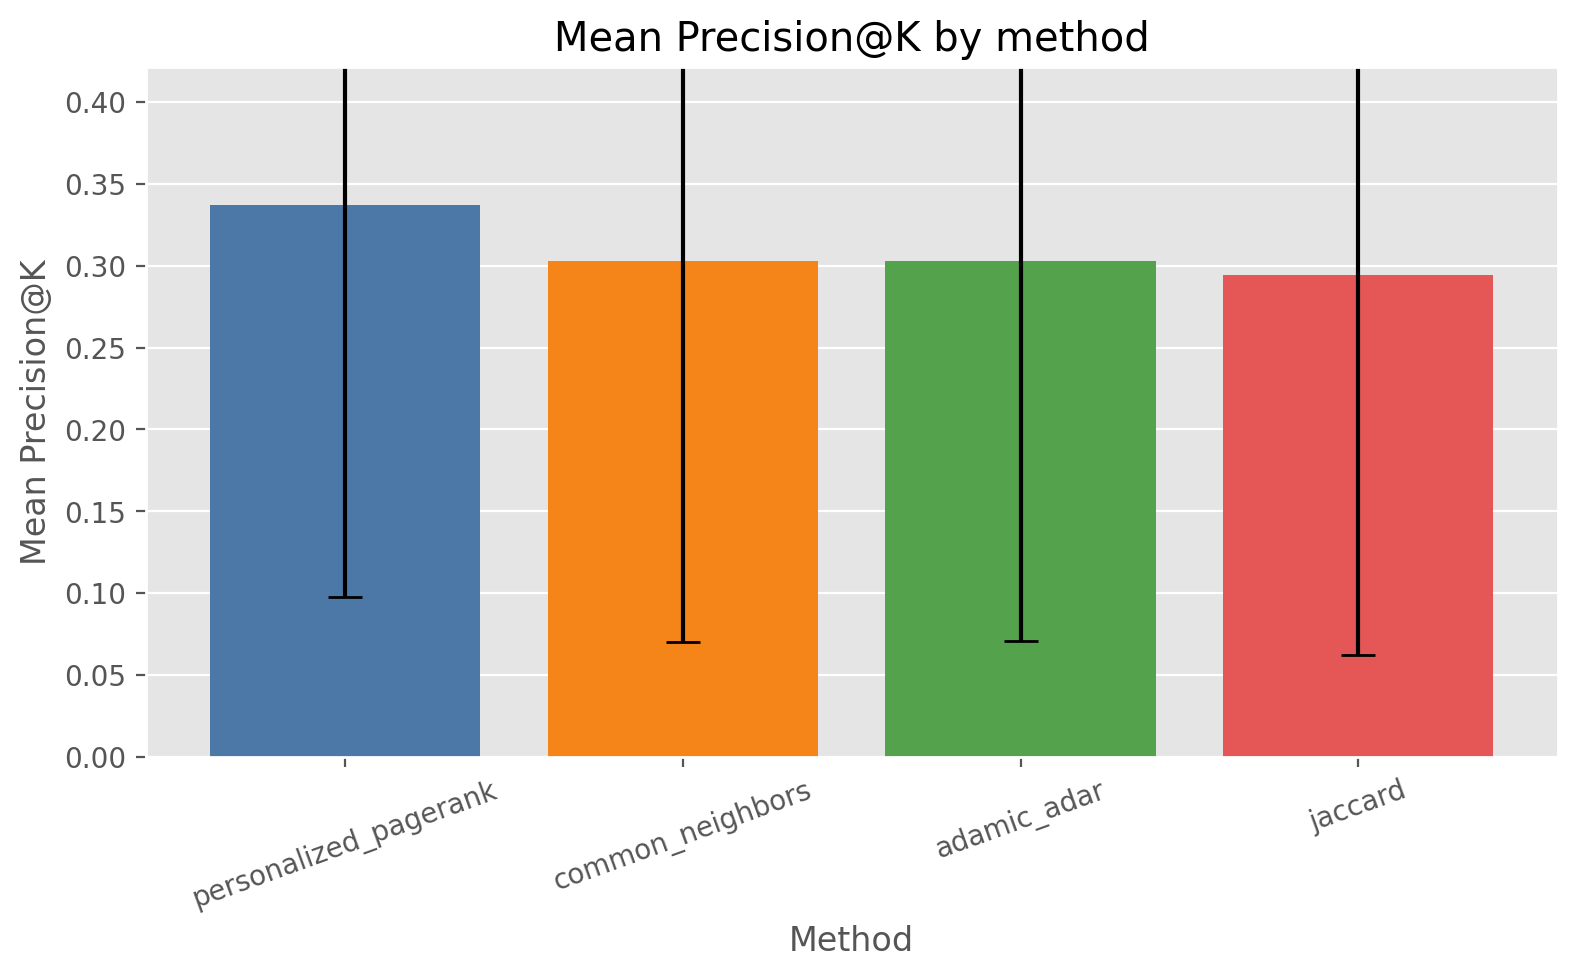
\includegraphics[width=0.72\textwidth]{../figures/precision_at_k_comparison}
  \caption{Mean Precision@10 by method with standard deviation error bars. Personalised PageRank clearly outperforms the three local similarity methods. Jaccard scores lowest because it penalises high-degree hub nodes that are genuine and important connectors in this network.}
  \label{fig:comparison}
\end{figure}

\begin{figure}[H]
  \centering
  \begin{subfigure}[b]{0.48\textwidth}
    \centering
    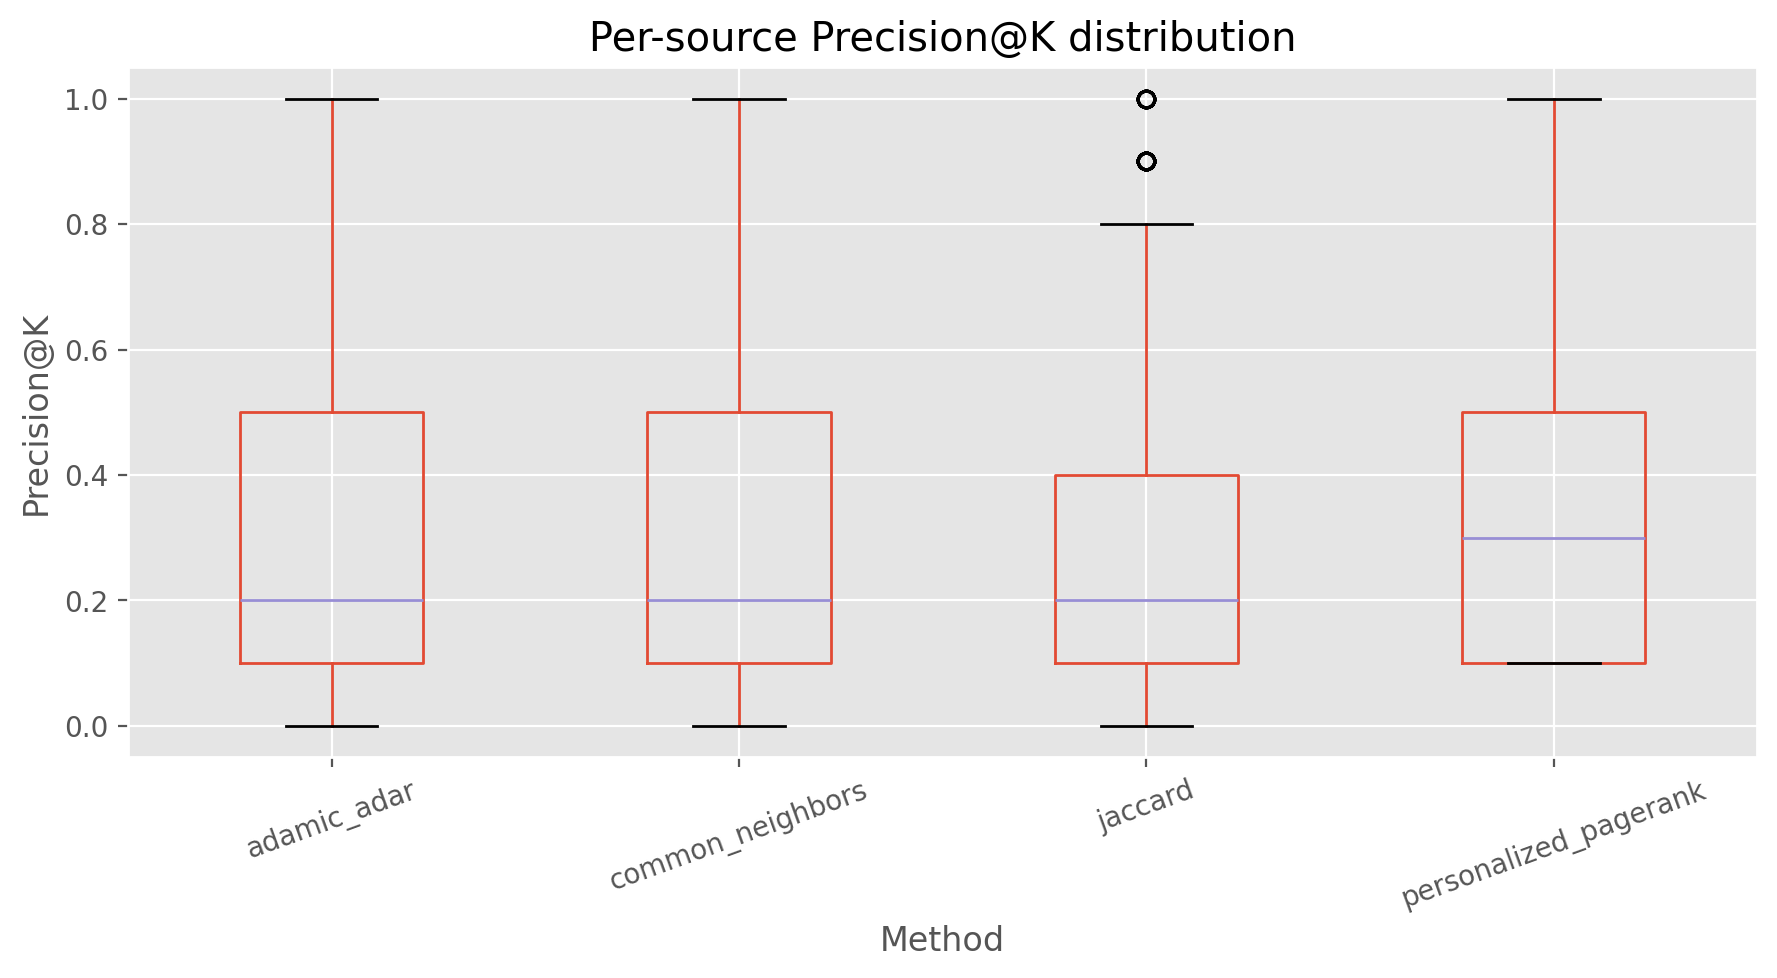
\includegraphics[width=\textwidth]{../figures/per_source_precision_boxplot}
    \caption{Per-source Precision@10 distribution (boxplot). The wide interquartile range shows high variance across nodes.}
    \label{fig:boxplot}
  \end{subfigure}
  \hfill
  \begin{subfigure}[b]{0.48\textwidth}
    \centering
    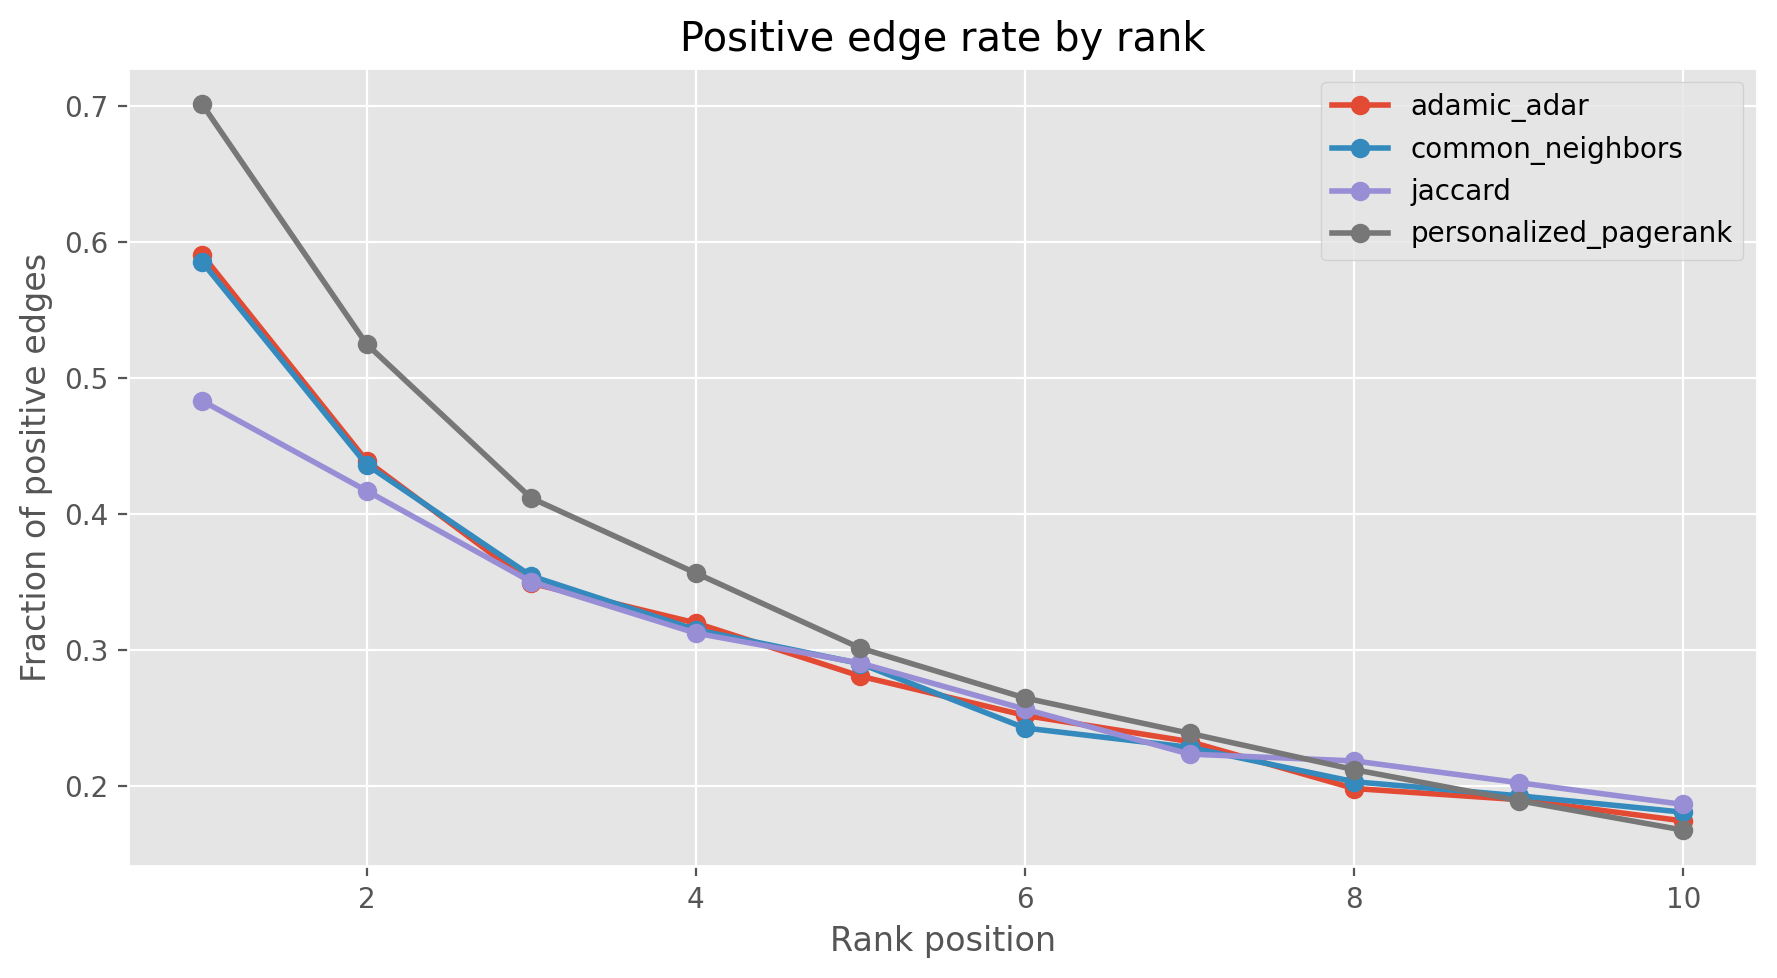
\includegraphics[width=\textwidth]{../figures/positive_rate_by_rank}
    \caption{Fraction of true positive edges at each rank position. All methods place true positives at earlier ranks.}
    \label{fig:rankquality}
  \end{subfigure}
  \caption{Per-source precision distribution (left) and rank quality analysis (right).}
  \label{fig:stability}
\end{figure}

\subsection{Precision@10 Bar Chart (Reproduced with TikZ)}

Figure~\ref{fig:tikzbar} reproduces the Precision@10 results as an inline TikZ chart for easy comparison with the random baseline.

\begin{figure}[H]
\centering
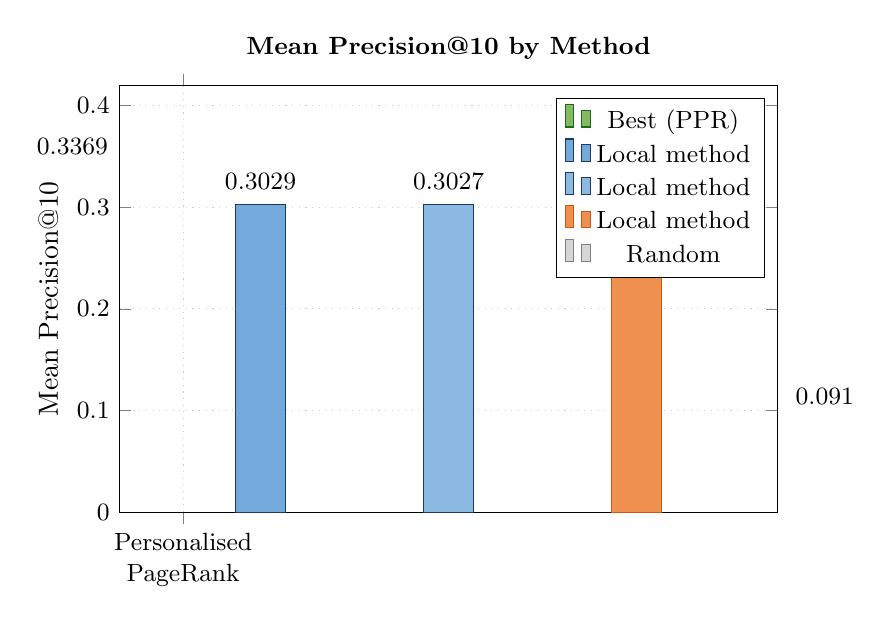
\begin{tikzpicture}
  \begin{axis}[
    ybar, bar width=18pt,
    width=0.82\textwidth, height=7cm,
    title={\small\textbf{Mean Precision@10 by Method}},
    ylabel={Mean Precision@10},
    symbolic x coords={PPR, CN, AA, Jaccard, Random},
    xtick=data,
    xticklabels={
      {Personalised\\PageRank},
      {Common\\Neighbours},
      {Adamic/\\Adar},
      {Jaccard},
      {Random\\(baseline)}
    },
    xticklabel style={align=center, font=\small},
    ymin=0, ymax=0.42,
    ytick={0, 0.1, 0.2, 0.3, 0.4},
    yticklabel style={font=\small},
    legend style={at={(0.98,0.97)}, anchor=north east, font=\small},
    nodes near coords,
    nodes near coords style={font=\small\bfseries, yshift=2pt},
    every node near coord/.append style={/pgf/number format/fixed,
      /pgf/number format/precision=4},
    enlarge x limits=0.12,
    grid=major, grid style={dotted, gray!40},
  ]
    \addplot[fill=ganttgreen!85, draw=darkgreen]
      coordinates {(PPR,0.3369)};
    \addplot[fill=ganttblue!85, draw=brandblue]
      coordinates {(CN,0.3029)};
    \addplot[fill=ganttblue!70, draw=brandblue]
      coordinates {(AA,0.3027)};
    \addplot[fill=ganttorange!85, draw=warnorange]
      coordinates {(Jaccard,0.2941)};
    \addplot[fill=midgray!80, draw=black!50]
      coordinates {(Random,0.091)};
    \legend{Best (PPR), Local method, Local method, Local method, Random}
  \end{axis}
\end{tikzpicture}
\caption{Precision@10 for all four methods and the random baseline. All graph-based methods are 3.2--3.7$\times$ better than random selection.}
\label{fig:tikzbar}
\end{figure}

\subsection{Relative Performance Analysis}

\begin{itemize}
  \item \textbf{PPR vs.\ Common Neighbours:} +3.4 percentage points improvement ($\approx$11\% relative gain). This gap reflects PPR's ability to follow multi-hop directed paths and assign relevance scores to nodes that have no direct shared neighbours with the source.
  \item \textbf{Common Neighbours vs.\ Adamic/Adar:} Nearly identical results (0.3029 vs.\ 0.3027). The inverse-log weighting in Adamic/Adar provides minimal additional discriminative power in this graph, likely because the heavy-tailed degree distribution means most shared neighbours are already medium-degree nodes where the log-degree values are similar across the shared set.
  \item \textbf{Jaccard:} The lowest scorer (0.2941). By normalising the neighbour count by the union size, Jaccard penalises high-degree administrators. However, in a trust network, these high-degree nodes are the genuine community connectors, and removing their signal hurts prediction quality.
\end{itemize}

\subsection{Per-Source Stability}

All methods show substantial standard deviation ($\approx$0.23), indicating that performance varies widely across source nodes (Figure~\ref{fig:boxplot}). Some nodes achieve Precision@10 close to 1.0, while others score near zero. This heterogeneity is expected: nodes with sparse training neighbourhoods give local similarity methods very little signal. PPR has slightly higher standard deviation (0.2389) because it leverages global paths and therefore benefits more from being in a well-connected region of the graph.

Figure~\ref{fig:rankquality} confirms that all methods consistently place true positive edges at earlier rank positions rather than later ones. This demonstrates that all four algorithms are genuinely learning the relevance structure of the graph, not just performing random selection.

% ============================================================
\section{Discussion}
\label{sec:discussion}
% ============================================================

\subsection{Why Personalised PageRank Outperforms Local Methods}

The Wikipedia Vote Network has a clear hub-and-spoke structure, where a small number of highly-trusted administrators received votes from a very large proportion of the community. Personalised PageRank naturally exploits this structure because it follows directed edges iteratively. If user $A$ voted for administrator $H$, and $H$ voted for many other administrators, then all of those administrators will receive indirect probability mass from $A$'s personalised random walk. This multi-hop inference is exactly the type of indirect reasoning that GraphRAG was designed to perform.

By contrast, Common Neighbours, Jaccard, and Adamic/Adar are limited to one-hop neighbourhood overlap. Two nodes that are two or three hops apart in the training graph receive a score of zero from these methods, even if they are strongly connected through a chain of intermediate nodes. In a knowledge graph where most entities are related through chains of intermediate nodes (not directly), this is a critical limitation.

\subsection{Connection to GraphRAG Context Retrieval}

The core claim of GraphRAG \cite{edge2024} is that graph-structured knowledge retrieval enables the discovery of contextually relevant information that flat keyword search cannot find. Our experiment provides a concrete, quantitative demonstration of this claim:

\begin{itemize}
  \item A \textbf{random retriever} achieves Precision@10 $\approx$ 0.091, providing roughly one relevant context node per 10-node window.
  \item \textbf{Personalised PageRank} achieves Precision@10 = 0.337, providing 3--4 relevant context nodes per 10-node window.
  \item This is a \textbf{3.7$\times$ improvement} over random selection using graph traversal alone, without any machine learning or document embeddings.
\end{itemize}

In a practical LLM pipeline, supplying 3--4 genuinely relevant context nodes (instead of 1) per context window would substantially reduce the probability of hallucination for questions that depend on indirect relationships, directly motivating the GraphRAG approach.

\begin{successbox}
\textbf{GraphRAG validation.} All four graph-based methods outperform random retrieval by a factor of 3.2--3.7$\times$, and Personalised PageRank outperforms the best local method by $\approx$11\% in relative terms. These results confirm that (1) graph structure is genuinely informative for context relevance, and (2) multi-hop traversal is more powerful than local neighbourhood similarity for this type of indirect relationship discovery task.
\end{successbox}

\subsection{Limitations}

\begin{limitbox}
\textbf{Limitations of this study.}
\begin{enumerate}
  \item \textbf{Simplified evaluation environment.} The test set consists of held-out edges from the same static graph, not real user queries in natural language. In a production GraphRAG system, queries come in free text and the relevant context may span different subgraphs.
  \item \textbf{Undirected projection for local methods.} Common Neighbours, Jaccard, and Adamic/Adar discard edge direction. Using direction-aware versions of these metrics might recover additional signal.
  \item \textbf{Static graph assumption.} Wikipedia's trust network evolves over time. A temporal split would more faithfully simulate a real deployment scenario, where the model must predict future connections from past data.
  \item \textbf{Partial node coverage.} Only 2,807 of the 7,115 nodes (39\%) appear in the test set and are evaluated. Nodes with no test edges are entirely absent from the Precision@10 computation.
  \item \textbf{No downstream LLM evaluation.} This project measures the quality of the retrieval module in isolation. The ultimate measure of GraphRAG quality is the improvement in LLM answer accuracy, which requires connecting the ranked candidates to an actual generation pipeline.
\end{enumerate}
\end{limitbox}

\subsection{Future Improvements}

\begin{itemize}
  \item \textbf{Ensemble scoring:} Normalise and combine all four scores into a single hybrid rank. Ensemble methods typically outperform any individual baseline \cite{libennowell2003}.
  \item \textbf{Additional metrics:} Add Recall@$K$ and AUC-ROC to measure whether all relevant nodes are retrieved, not only whether the top-$K$ items are precise.
  \item \textbf{GNN-based predictor:} Replace heuristic scoring with a trained model such as GraphSAGE or a Graph Attention Network (GAT), using node degree and structural features as inputs.
  \item \textbf{Temporal split:} Use node ID ordering as a proxy for account creation time to create a more realistic time-based evaluation split.
  \item \textbf{End-to-end integration:} Connect the ranked candidate nodes to a Claude or GPT API and measure the improvement in answer quality on indirect-relationship questions.
\end{itemize}

% ============================================================
\section{Conclusion}
\label{sec:conclusion}
% ============================================================

This report presented a simplified GraphRAG retrieval module implemented on the Wikipedia Vote Network, framed as a link prediction problem. We implemented and evaluated four graph-based scoring algorithms --- Common Neighbours, Jaccard Coefficient, Adamic/Adar Index, and Personalised PageRank --- using Precision@10 on a held-out 20\% test set with stratified negative sampling.

The main findings of this project are as follows:

\begin{enumerate}
  \item All four graph-based methods substantially outperform random retrieval, confirming that graph structure provides real, useful information for identifying relevant context nodes.
  \item \textbf{Personalised PageRank achieves the highest Precision@10 of 0.3369}, which is 3.7$\times$ better than the random baseline and approximately 11\% better than the best local similarity method (Common Neighbours at 0.3029). Its advantage comes from following multi-hop directed paths, which is the fundamental capability needed for indirect relationship discovery.
  \item Common Neighbours and Adamic/Adar produce nearly identical results (0.3029 vs.\ 0.3027), showing that the inverse-log weighting of Adamic/Adar adds minimal discriminative power in this heavy-tailed network.
  \item Jaccard scores the lowest (0.2941) because its normalisation penalises high-degree hub nodes that are actually meaningful connectors in this trust network.
  \item All methods show high variance across source nodes (std $\approx$ 0.23), indicating that graph retrieval quality is uneven and depends heavily on a node's position within the network.
\end{enumerate}

These results provide concrete, quantitative evidence that graph-structured retrieval --- particularly multi-hop traversal via Personalised PageRank --- is significantly more effective than flat keyword or similarity-based approaches for discovering indirect relationships. This directly validates the core motivation of the GraphRAG approach: by organising knowledge as a graph, a retrieval module can surface the contextual connections that LLMs need to answer complex, multi-hop queries without hallucinating.

\begin{callout}
\textbf{Final takeaway.} Personalised PageRank delivers 3.4 genuinely relevant context nodes per 10-node window on average --- 3.7$\times$ more than random selection. In a production GraphRAG system, this improvement in retrieval precision would meaningfully reduce LLM hallucination for questions about indirect relationships, making graph-structured retrieval a practically valuable component of any knowledge-intensive AI application.
\end{callout}

% ============================================================
%  REFERENCES
% ============================================================
\newpage
\renewcommand{\refname}{References}
\addcontentsline{toc}{section}{References}

\makeatletter
\renewcommand\@biblabel[1]{}
\makeatother

\begin{thebibliography}{99}

\bibitem{edge2024}
\hangindent=36pt \hangafter=1
D. Edge, H. Trinh, N. Cheng, J. Bradley, A. Chao, A. Mody, S. Truitt, and J. Larson, ``From local to global: A graph RAG approach to query-focused summarization,'' \textit{arXiv preprint arXiv:2404.16130}, 2024.

\bibitem{pan2024}
\hangindent=36pt \hangafter=1
S. Pan, L. Luo, Y. Wang, C. Chen, J. Wang, and X. Wu, ``Unifying large language models and knowledge graphs: A roadmap,'' \textit{IEEE Transactions on Knowledge and Data Engineering}, 2024. doi: 10.1109/TKDE.2024.3352100

\bibitem{lewis2020}
\hangindent=36pt \hangafter=1
P. Lewis, E. Perez, A. Piktus, F. Petroni, V. Karpukhin, N. Goyal, H. K\"{u}ttler, M. Lewis, W. Yih, T. Rockt\"{a}schel, S. Riedel, and D. Kiela, ``Retrieval-augmented generation for knowledge-intensive NLP tasks,'' in \textit{Advances in Neural Information Processing Systems}, vol. 33, pp. 9459--9474, 2020.

\bibitem{libennowell2003}
\hangindent=36pt \hangafter=1
D. Liben-Nowell and J. Kleinberg, ``The link prediction problem for social networks,'' in \textit{Proceedings of the 12th International Conference on Information and Knowledge Management (CIKM)}, pp. 556--559, 2003.

\bibitem{adamic2003}
\hangindent=36pt \hangafter=1
L. A. Adamic and E. Adar, ``Friends and neighbors on the web,'' \textit{Social Networks}, vol. 25, no. 3, pp. 211--230, 2003.

\bibitem{page1999}
\hangindent=36pt \hangafter=1
L. Page, S. Brin, R. Motwani, and T. Winograd, ``The PageRank citation ranking: Bringing order to the web,'' Technical Report 1999-66, Stanford InfoLab, 1999.

\bibitem{snap2014}
\hangindent=36pt \hangafter=1
J. Leskovec and A. Krevl, ``{SNAP} datasets: {Stanford} large network dataset collection,'' 2014. [Online]. Available: http://snap.stanford.edu/data

\bibitem{hamilton2017}
\hangindent=36pt \hangafter=1
W. Hamilton, Z. Ying, and J. Leskovec, ``Inductive representation learning on large graphs,'' in \textit{Advances in Neural Information Processing Systems}, vol. 30, 2017.

\end{thebibliography}

% ============================================================
%  APPENDICES
% ============================================================
\newpage
\begin{appendices}

% ---- Appendix A: Dashboard Screenshots ----------------------
\section{Results Dashboard Screenshots}
\label{app:dashboard}

The following screenshots are taken from the project's interactive HTML results dashboard (\texttt{reports/dashboard.html}). The dashboard summarises the dataset statistics, pipeline architecture, algorithm descriptions, Precision@10 results table, and all four analysis figures in a single self-contained page that can be opened in any web browser without a server.

\begin{figure}[H]
  \centering
  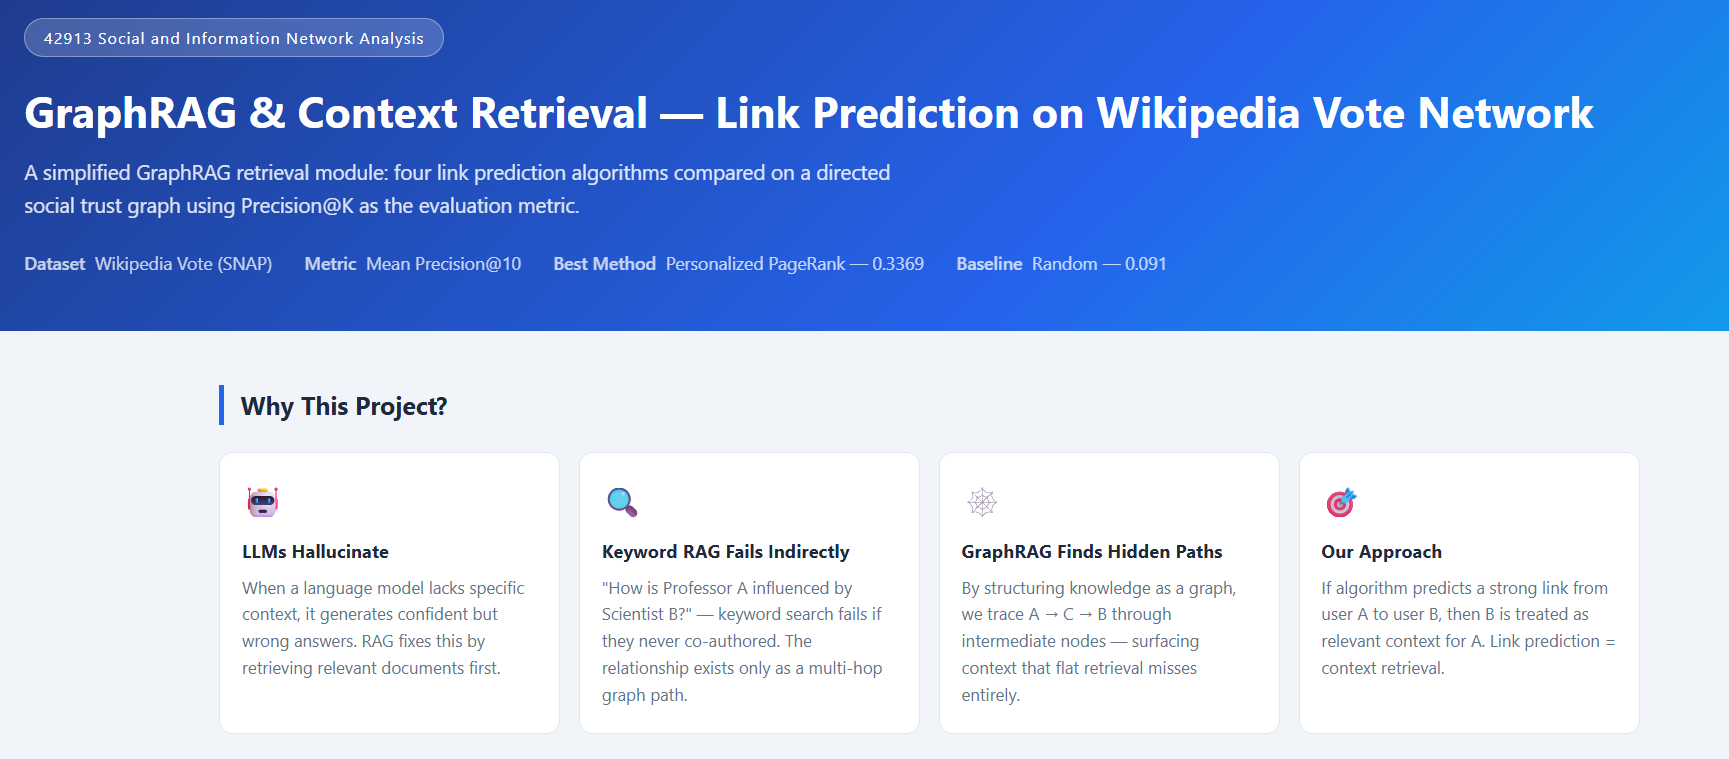
\includegraphics[width=\linewidth]{Imagens/dataset1_dashboard1}
  \caption{Dashboard --- header section showing the project title, course information, and key result summary. The header cards display: best method (Personalised PageRank, P@10 = 0.3369), dataset name, and random baseline comparison.}
  \label{fig:dash1}
\end{figure}

\begin{figure}[H]
  \centering
  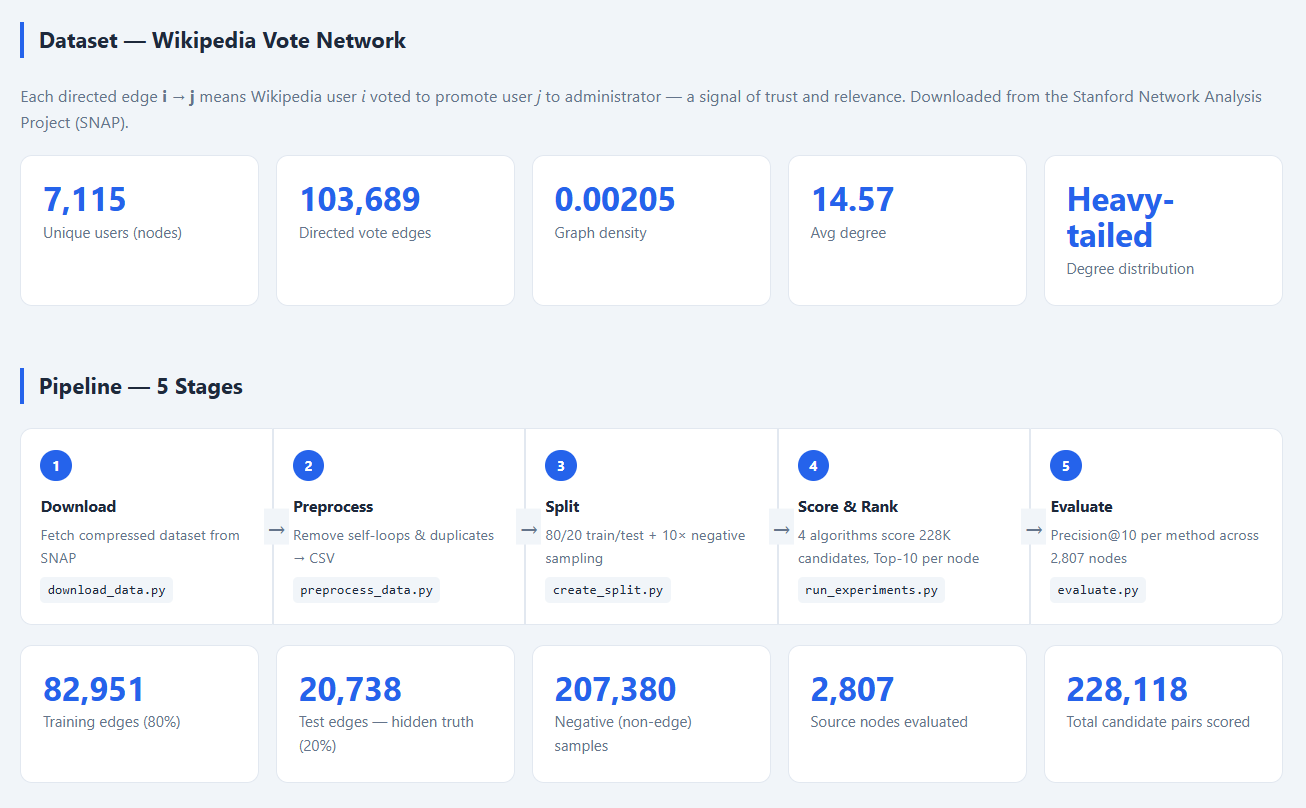
\includegraphics[width=\linewidth]{Imagens/dataset1_dashboard2}
  \caption{Dashboard --- ``Why This Project?'' motivation cards and dataset statistics. The four motivation cards explain the LLM hallucination problem, the failure of keyword RAG for indirect queries, the GraphRAG solution, and our project approach.}
  \label{fig:dash2}
\end{figure}

\begin{figure}[H]
  \centering
  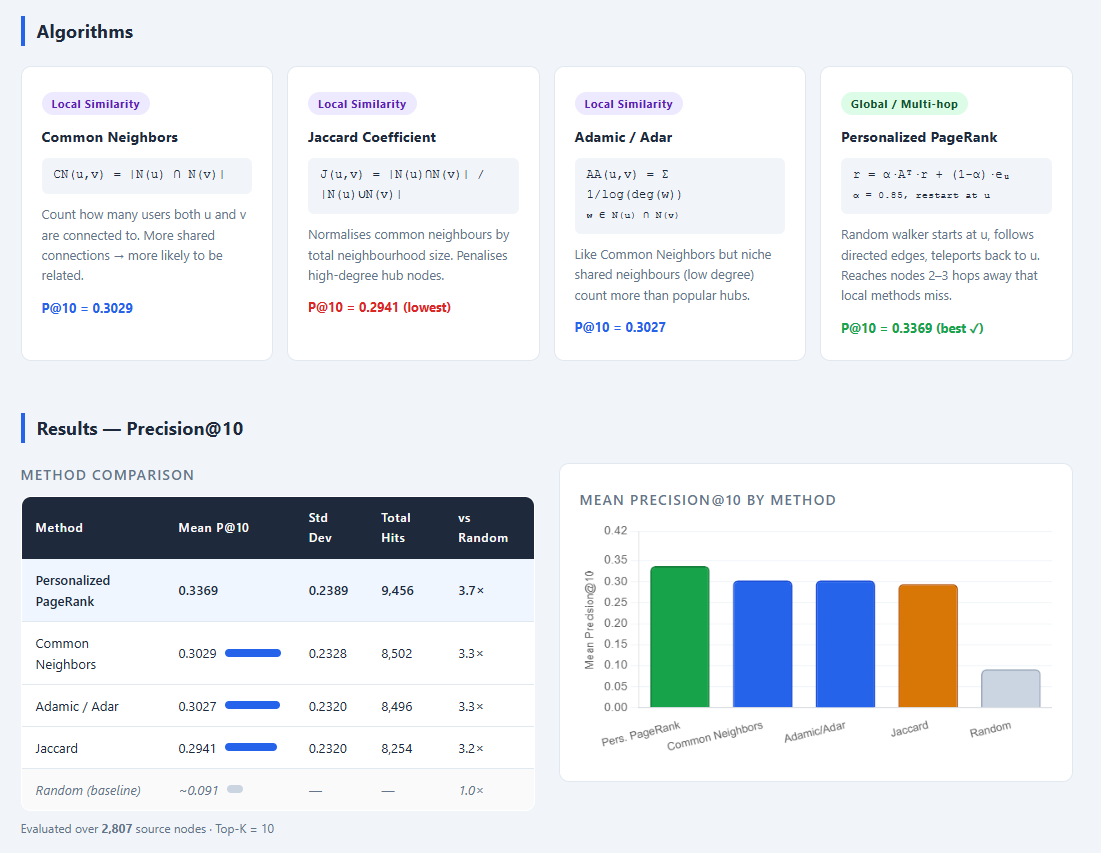
\includegraphics[width=\linewidth]{Imagens/dataset1_dashboard3}
  \caption{Dashboard --- pipeline steps and algorithm cards. The five pipeline steps show the end-to-end workflow from download to evaluation. The four algorithm cards display formulas and Precision@10 scores colour-coded by performance.}
  \label{fig:dash3}
\end{figure}

\begin{figure}[H]
  \centering
  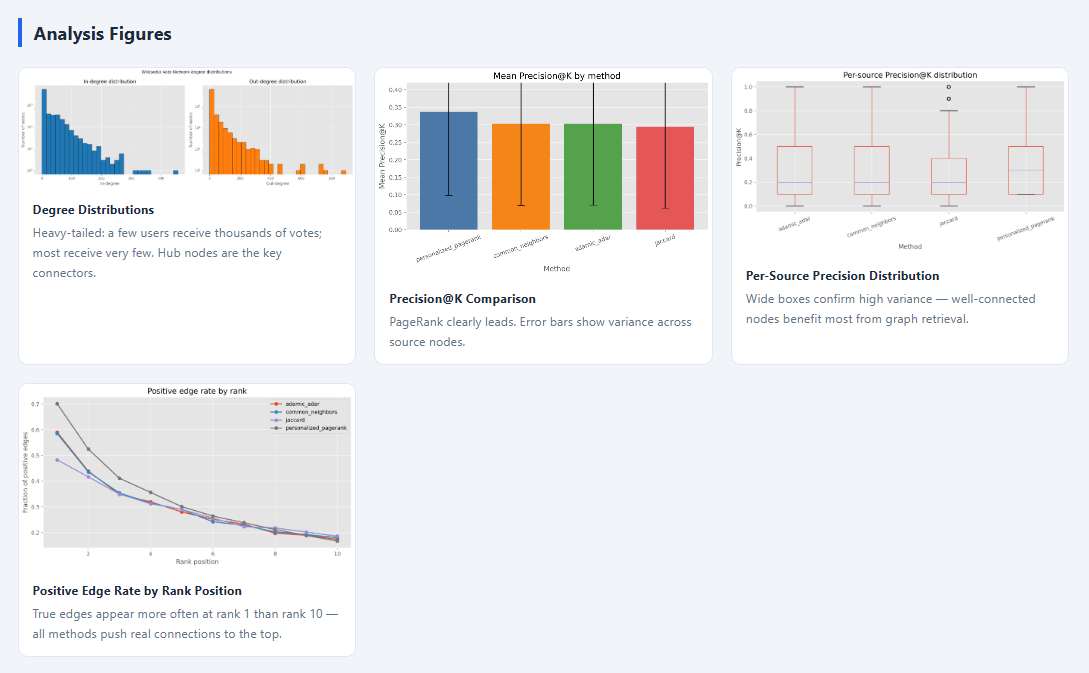
\includegraphics[width=\linewidth]{Imagens/dataset1_dashboard4}
  \caption{Dashboard --- results table and interactive Precision@10 bar chart (rendered using Chart.js). The table shows mean P@10, standard deviation, total hits, and performance relative to the random baseline for all four methods.}
  \label{fig:dash4}
\end{figure}

\begin{figure}[H]
  \centering
  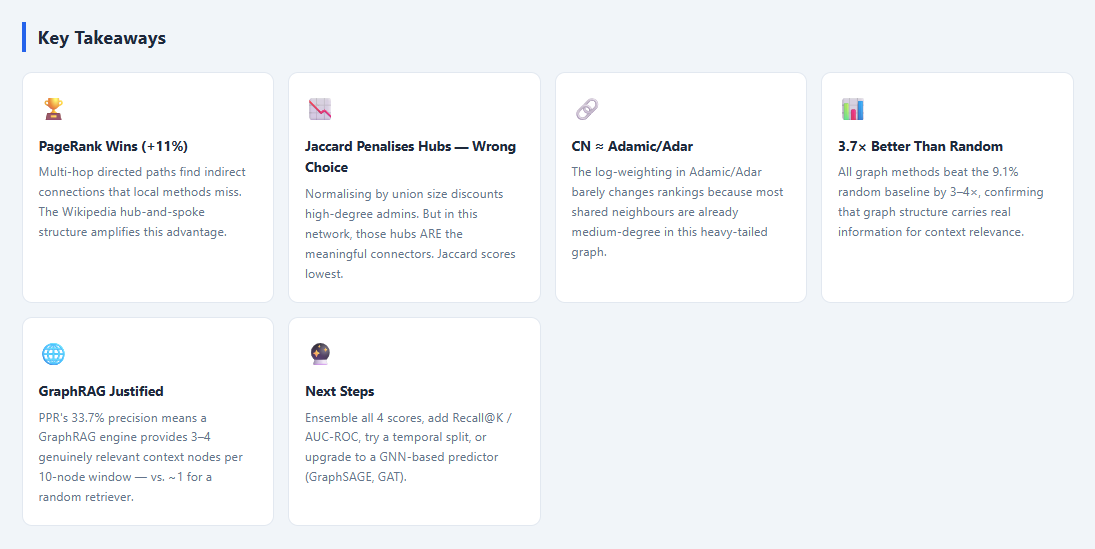
\includegraphics[width=\linewidth]{Imagens/dataset1_dashboard5}
  \caption{Dashboard --- analysis figures section showing the four PNG charts embedded inline: degree distributions, precision comparison, per-source boxplot, and positive edge rate by rank position.}
  \label{fig:dash5}
\end{figure}

% ---- Appendix B: Repository Structure ----------------------
\section{Repository Structure and Reproducibility}
\label{app:repo}

The complete project is available in the GitHub repository. All results can be reproduced by running the following five commands in order from the project root directory:

\begin{enumerate}
  \item \texttt{python scripts/download\_data.py} \hfill\textit{Download wiki-Vote.txt from SNAP}
  \item \texttt{python scripts/preprocess\_data.py} \hfill\textit{Clean edges to CSV}
  \item \texttt{python scripts/create\_split.py -{}-test-size 0.2 -{}-negatives-per-positive 10 -{}-seed 42}
  \item \texttt{python scripts/run\_experiments.py -{}-top-k 10} \hfill\textit{Score, rank, and evaluate}
  \item Open \texttt{notebooks/02\_results\_analysis.ipynb} \hfill\textit{Generate all figures}
\end{enumerate}

\begin{table}[H]
  \centering
  \caption{Key output files generated by the pipeline.}
  \label{tab:outputs}
  \small
  \begin{tabular}{l l}
    \hline
    \rowcolor{brandblue}
    \theadfont File & \theadfont Description \\
    \hline
    \rowcolor{lightblue}
    \texttt{data/processed/graph\_edges.csv}         & Cleaned edge list (103,689 rows) \\
    \texttt{data/splits/train\_edges.csv}            & Training graph (82,951 edges) \\
    \rowcolor{lightblue}
    \texttt{data/splits/test\_edges.csv}             & Hidden test edges (20,738 edges) \\
    \texttt{data/splits/negative\_samples.csv}       & Sampled non-edges (207,380 rows) \\
    \rowcolor{lightblue}
    \texttt{results/predictions/scored\_candidates.csv} & All candidate pairs with 4 scores \\
    \texttt{results/predictions/topk\_predictions.csv}  & Top-10 predictions per source per method \\
    \rowcolor{lightblue}
    \texttt{results/metrics/evaluation\_summary.csv} & Precision@10 per method (tracked in git) \\
    \texttt{reports/figures/*.png}                   & Four analysis charts for the report \\
    \rowcolor{lightblue}
    \texttt{reports/dashboard.html}                  & Self-contained HTML results dashboard \\
    \hline
  \end{tabular}
\end{table}

\end{appendices}

\end{document}
